
\documentclass[letterpaper,hide notes,xcolor={table,svgnames},pdftex,10pt]{beamer}
\def\showexamples{t}

\usecolortheme{crane}
\setbeamertemplate{navigation symbols}{}

\usetheme{MyPittsburgh}
\usepackage{hyperref}
\usepackage{graphicx,xspace}
\usepackage[normalem]{ulem}
\usepackage{multicol}
\usepackage{amsmath,amssymb,amsthm,graphicx,xspace}
\newcommand\SF[1]{$\bigstar$\footnote{SF: #1}}

\usepackage[sfdefault,lf]{carlito}
\usepackage[T1]{fontenc}
\usepackage[scaled]{beramono}
\usepackage{tikzpagenodes}
\newcommand{\Rplus}{\protect\hspace{-.1em}\protect\raisebox{.35ex}{\small{\small\textbf{+}}}}
\newcommand{\Cpp}{\mbox{C\Rplus\Rplus}\xspace}

\newcounter{tmpnumSlide}
\newcounter{tmpnumNote}

\newcommand\mnote[1]{%
	\addtocounter{tmpnumSlide}{1}
	\ifdefined\showcues {~\tiny\fbox{\arabic{tmpnumSlide}}}\fi
	\note{\setlength{\parskip}{1ex}\addtocounter{tmpnumNote}{1}\textbf{\Large \arabic{tmpnumNote}:} {#1\par}}}

\newcommand\mmnote[1]{\note{\setlength{\parskip}{1ex}#1\par}}


\newcommand\mquestion[2]{{~\color{red}\fbox{?}}\note{\setlength{\parskip}{1ex}\par{\Large \textbf{?}} #1} \note{\setlength{\parskip}{1ex}\par{\Large \textbf{A}} #2\par}\ifdefined \presentationonly \pause \fi}

\newcommand\blackboard[1]{%
	\ifdefined   \showblackboard
		{#1}
	\else {\begin{center} \fbox{\colorbox{blue!30}{%
						\begin{minipage}{.95\linewidth}%
							\hspace{\stretch{1}} Some space intentionally left blank; done at the blackboard.%
						\end{minipage}}}\end{center}}%
	\fi%
}

\usepackage{listings}
\lstset{%
	keywordstyle=\bfseries,
	aboveskip=15pt,
	belowskip=15pt,
	captionpos=b,
	identifierstyle=\ttfamily,
	frame=lines,
	numbers=left, basicstyle=\scriptsize, numberstyle=\tiny, stepnumber=0, numbersep=2pt}

\usepackage{siunitx}
\newcommand\sius[1]{\num[group-separator = {,}]{#1}\si{\micro\second}}
\newcommand\sims[1]{\num[group-separator = {,}]{#1}\si{\milli\second}}
\newcommand\sins[1]{\num[group-separator = {,}]{#1}\si{\nano\second}}
\sisetup{group-separator = {,}, group-digits = true}

%% -------------------- tikz --------------------
\usepackage{tikz}
\usetikzlibrary{positioning}
\usetikzlibrary{arrows,backgrounds,automata,decorations.shapes,decorations.pathmorphing,decorations.markings,decorations.text}

\tikzstyle{place}=[circle,draw=blue!50,fill=blue!20,thick, inner sep=0pt,minimum size=6mm]
\tikzstyle{transition}=[rectangle,draw=black!50,fill=black!20,thick, inner sep=0pt,minimum size=4mm]

\tikzstyle{block}=[rectangle,draw=black, thick, inner sep=5pt]
\tikzstyle{bullet}=[circle,draw=black, fill=black, thin, inner sep=2pt]

\tikzstyle{pre}=[<-,shorten <=1pt,>=stealth',semithick]
\tikzstyle{post}=[->,shorten >=1pt,>=stealth',semithick]
\tikzstyle{bi}=[<->,shorten >=1pt,shorten <=1pt, >=stealth',semithick]

\tikzstyle{mut}=[-,>=stealth',semithick]

\tikzstyle{treereset}=[dashed,->, shorten >=1pt,>=stealth',thin]

\usepackage{ifmtarg}
\usepackage{xifthen}
\makeatletter
% new counter to now which frame it is within the sequence
\newcounter{multiframecounter}
% initialize buffer for previously used frame title
\gdef\lastframetitle{\textit{undefined}}
% new environment for a multi-frame
\newenvironment{multiframe}[1][]{%
	\ifthenelse{\isempty{#1}}{%
		% if no frame title was set via optional parameter,
		% only increase sequence counter by 1
		\addtocounter{multiframecounter}{1}%
	}{%
		% new frame title has been provided, thus
		% reset sequence counter to 1 and buffer frame title for later use
		\setcounter{multiframecounter}{1}%
		\gdef\lastframetitle{#1}%
	}%
	% start conventional frame environment and
	% automatically set frame title followed by sequence counter
	\begin{frame}%
		\frametitle{\lastframetitle~{\normalfont(\arabic{multiframecounter})}}%
		}{%
	\end{frame}%
}
\makeatother

\makeatletter
\newdimen\tu@tmpa%
\newdimen\ydiffl%
\newdimen\xdiffl%
\newcommand\ydiff[2]{%
	\coordinate (tmpnamea) at (#1);%
	\coordinate (tmpnameb) at (#2);%
	\pgfextracty{\tu@tmpa}{\pgfpointanchor{tmpnamea}{center}}%
	\pgfextracty{\ydiffl}{\pgfpointanchor{tmpnameb}{center}}%
	\advance\ydiffl by -\tu@tmpa%
}
\newcommand\xdiff[2]{%
	\coordinate (tmpnamea) at (#1);%
	\coordinate (tmpnameb) at (#2);%
	\pgfextractx{\tu@tmpa}{\pgfpointanchor{tmpnamea}{center}}%
	\pgfextractx{\xdiffl}{\pgfpointanchor{tmpnameb}{center}}%
	\advance\xdiffl by -\tu@tmpa%
}
\makeatother
\newcommand{\copyrightbox}[3][r]{%
	\begin{tikzpicture}%
		\node[inner sep=0pt,minimum size=2em](ciimage){#2};
		\usefont{OT1}{phv}{n}{n}\fontsize{4}{4}\selectfont
		\ydiff{ciimage.south}{ciimage.north}
		\xdiff{ciimage.west}{ciimage.east}
		\ifthenelse{\equal{#1}{r}}{%
			\node[inner sep=0pt,right=1ex of ciimage.south east,anchor=north west,rotate=90]%
			{\raggedleft\color{black!50}\parbox{\the\ydiffl}{\raggedright{}#3}};%
		}{%
			\ifthenelse{\equal{#1}{l}}{%
				\node[inner sep=0pt,right=1ex of ciimage.south west,anchor=south west,rotate=90]%
				{\raggedleft\color{black!50}\parbox{\the\ydiffl}{\raggedright{}#3}};%
			}{%
				\node[inner sep=0pt,below=1ex of ciimage.south west,anchor=north west]%
				{\raggedleft\color{black!50}\parbox{\the\xdiffl}{\raggedright{}#3}};%
			}
		}
	\end{tikzpicture}
}


%% --------------------

%\usepackage[excludeor]{everyhook}
%\PushPreHook{par}{\setbox0=\lastbox\llap{MUH}}\box0}

%\vspace*{\stretch{1}

%\setbox0=\lastbox \llap{\textbullet\enskip}\box0}

\setlength{\parskip}{\fill}

\newcommand\noskips{\setlength{\parskip}{1ex}}
\newcommand\doskips{\setlength{\parskip}{\fill}}

\newcommand\xx{\par\vspace*{\stretch{1}}\par}
\newcommand\xxs{\par\vspace*{2ex}\par}
\newcommand\tuple[1]{\langle #1 \rangle}
\newcommand\code[1]{{\sf \footnotesize #1}}
\newcommand\ex[1]{\uline{Example:} \ifdefined \presentationonly \pause \fi
	\ifdefined\showexamples#1\xspace\else{\uline{\hspace*{2cm}}}\fi}

\newcommand\ceil[1]{\lceil #1 \rceil}


\AtBeginSection[]
{
	\begin{frame}
		\frametitle{Outline}
		\tableofcontents[currentsection]
	\end{frame}
}



\pgfdeclarelayer{edgelayer}
\pgfdeclarelayer{nodelayer}
\pgfsetlayers{edgelayer,nodelayer,main}

\tikzstyle{none}=[inner sep=0pt]
\tikzstyle{rn}=[circle,fill=Red,draw=Black,line width=0.8 pt]
\tikzstyle{gn}=[circle,fill=Lime,draw=Black,line width=0.8 pt]
\tikzstyle{yn}=[circle,fill=Yellow,draw=Black,line width=0.8 pt]
\tikzstyle{empty}=[circle,fill=White,draw=Black]
\tikzstyle{bw} = [rectangle, draw, fill=blue!20,
text width=4em, text centered, rounded corners, minimum height=2em]

\newcommand{\CcNote}[1]{% longname
	This work is licensed under the \textit{Creative Commons #1 3.0 License}.%
}
\newcommand{\CcImageBy}[1]{%
	\includegraphics[scale=#1]{creative_commons/cc_by_30.pdf}%
}
\newcommand{\CcImageSa}[1]{%
	\includegraphics[scale=#1]{creative_commons/cc_sa_30.pdf}%
}
\newcommand{\CcImageNc}[1]{%
	\includegraphics[scale=#1]{creative_commons/cc_nc_30.pdf}%
}
\newcommand{\CcGroupBySa}[2]{% zoom, gap
	\CcImageBy{#1}\hspace*{#2}\CcImageNc{#1}\hspace*{#2}\CcImageSa{#1}%
}
\newcommand{\CcLongnameByNcSa}{Attribution-NonCommercial-ShareAlike}

\newenvironment{changemargin}[1]{% 
	\begin{list}{}{% 
		\setlength{\topsep}{0pt}% 
		\setlength{\leftmargin}{#1}% 
		\setlength{\rightmargin}{1em}
		\setlength{\listparindent}{\parindent}% 
		\setlength{\itemindent}{\parindent}% 
		      \setlength{\parsep}{\parskip}% 
		      }% 
		\item[]}{\end{list}}




\title{Lecture 29 --- Asynchronous I/O with select, poll }

\author{Jeff Zarnett \\ \small \texttt{jzarnett@uwaterloo.ca}}
\institute{Department of Electrical and Computer Engineering \\
	University of Waterloo}
\date{\today}


\begin{document}

\begin{frame}
	\titlepage

\end{frame}


\begin{frame}
	\frametitle{Read Me A Book}

	As we discussed much earlier, the \texttt{read} call is blocking, as expected.

	So, your program waits for the I/O operation to be complete before continuing on to the next statements (whatever they are).

	This is sometimes, but not always, sensible.

	If you need the data in the next statement, you can't go on until it's there.

\end{frame}


\begin{frame}
	\frametitle{Waiting for the Bus}

	\begin{center}
		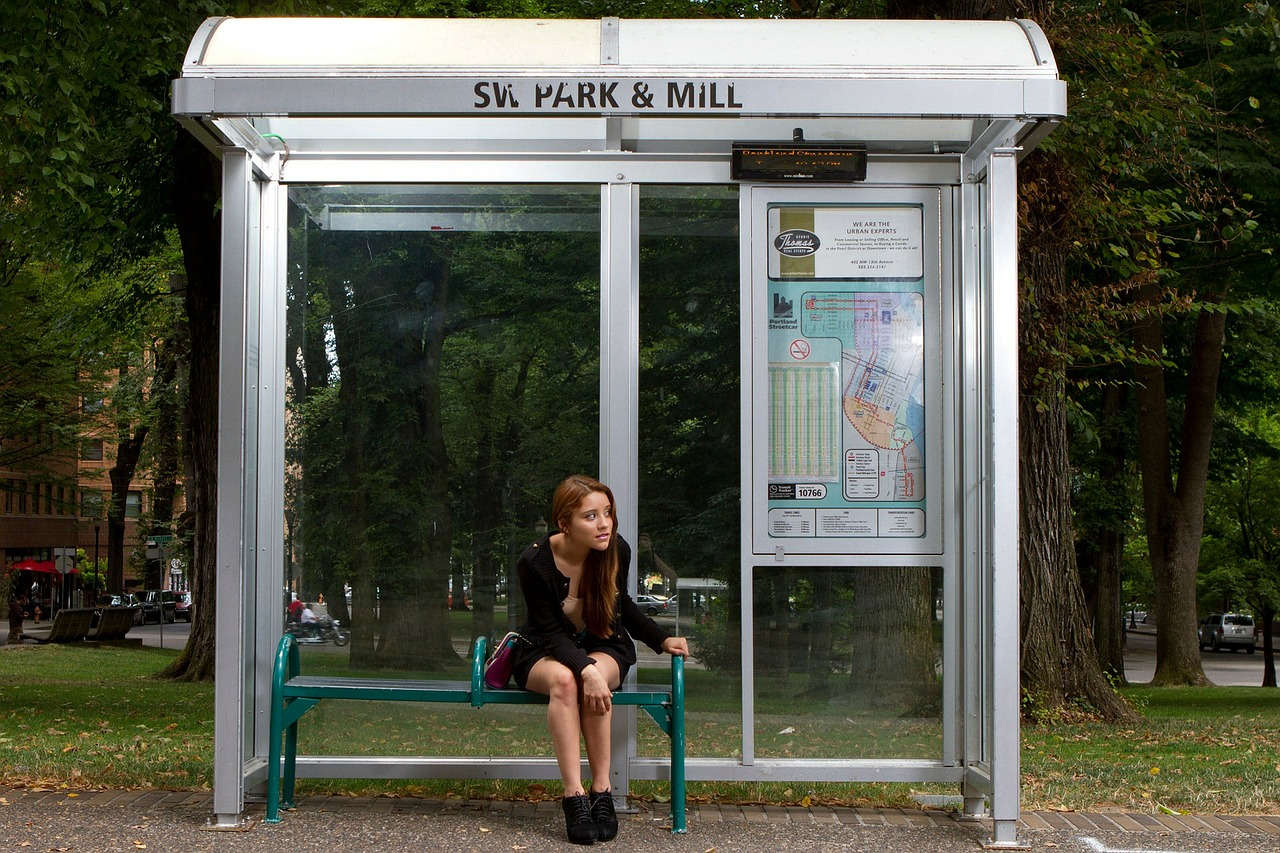
\includegraphics[width=0.9\textwidth]{images/thebus.jpg}
	\end{center}

	If you are waiting for the bus, do you stare off blankly into space while waiting for it to arrive?

\end{frame}

\begin{frame}
	\frametitle{Haha, As If}

	\begin{center}
		
\includegraphics[width=0.9\textwidth]{images/textbus.png}
	\end{center}

	More likely you pull out your phone and start to use it for something.

\end{frame}

\begin{frame}
	\frametitle{We Have Threads!}

	Our main solution until now is threads!

	If one thread gets blocked on the I/O the other ones can continue and is fine.

	But maybe you don't want to use threads, or maybe you can't for a reason?

	Some languages give you no choice, like JavaScript!

\end{frame}


\begin{frame}[fragile]
	\frametitle{Jump To It}

	The simplest example:

	\begin{lstlisting}[language=C]
int fd = open( "example.txt", O_RDONLY | O_NONBLOCK );
int bytes_read = read( fd, buffer, num_bytes ); /* Returns instantly! */
close( fd );
\end{lstlisting}

	That was easy, right?

\end{frame}


\begin{frame}
	\frametitle{There's a Catch}

	If we opened the file in non-blocking, the \texttt{read} call returns instantly.

	Whether or not results are ready.

	The \texttt{O\_NONBLOCK} option is not helpful, because this call says we should not wait for data when there is no data available.

	But a file \textit{always} has data available.

	Do we know any scenarios where we don't have data always available?

\end{frame}


\begin{frame}[fragile]
	\frametitle{Sockets!}

	If we haven't received data, we'd get blocked waiting for some data to arrive.

	But we can change that behaviour on a socket if we wish, by setting the socket to be nonblocking:

	\begin{lstlisting}[language=C]
sockfd = socket( PF_INET, SOCK_STREAM, 0 );
fcntl( sockfd, F_SETFL, O_NONBLOCK );
\end{lstlisting}

	This means that calls to \texttt{accept()}, \texttt{recv()}, or \texttt{recvfrom()} would not block.

\end{frame}

\begin{frame}
	\frametitle{Nonblocking Socket}

	If you call those and there's no data to receive, you get back a return value of \texttt{-1} and \texttt{errno} is going to be either \texttt{EAGAIN} or \texttt{EWOULDBLOCK}.

	Sadly, the specification does not say which it would be, so the fully correct approach is to check for both.

	Not great, but it's how we are sure.

\end{frame}


\begin{frame}
	\frametitle{Server Setup}

	You are writing a server application that's going to listen on several sockets.

	This is a common enough scenario.

	You could have different threads listening on their individual sockets but -- see the reasoning above as to why we might not have that option.

	And we no longer have to!

\end{frame}


\begin{frame}
	\frametitle{Wasting Our Time?}

	But if we are a server and there aren't any incoming requests, what exactly are we supposed to do with our time?

	If we just poll each socket using, for example, \texttt{accept()}, this amounts to tight polling and is CPU intensive and wastes the CPU's time.

	What we need is a third option.
\end{frame}


\begin{frame}
	\frametitle{Select...}

	\begin{center}
		
\includegraphics[width=0.5\textwidth]{images/sarahconnor.png}
	\end{center}

\end{frame}

\begin{frame}
	\frametitle{Select!}

	The third option is called \texttt{select()} -- it allows us to monitor a group of sockets, telling us about the state of each of them.

	A socket could be ready for a read, ready for a write (of small size), or whether an exception has occurred.

	So actually, select works on three sets of sockets...

\end{frame}

\begin{frame}[fragile]
	\frametitle{Select Definition}

	\begin{lstlisting}[language=C]
 int select( int nfds, fd_set *readfds, fd_set *writefds, 
     fd_set *exceptfds, struct timeval *timeout );
\end{lstlisting}

	If we call this function, we'll get blocked until something happens on one of the sockets so that it becomes ``ready''... or until we reach a timeout.

	While blocked, we could also get interrupted by something (e.g., a signal).

	\texttt{nfds}: the value of the highest number file descriptor plus 1.

	\texttt{timeout}: pretty self-explanatory.

	What about the \texttt{fd\_set} parameters?

\end{frame}

\begin{frame}
	\frametitle{File Descriptor Sets}

	The \texttt{fd\_set} structure can have up to 1024 file descriptors, and is actually implemented as a bitfield.

	The kernel can stop looking once we reached the last one.

	Well, we were going to have to figure out what the \texttt{fd\_set} means anyway.

	It represents a set of file descriptors, just as the name says.

\end{frame}

\begin{frame}[fragile]
	\frametitle{File Descriptor Sets}

	\begin{lstlisting}
void FD_ZERO( fd_set *set ); /* Clear the set */
void FD_SET( int fd, fd_set *set ); /* Add fd to the set */
void FD_CLR( int fd, fd_set *set ); /* Remove fd from the set */
int  FD_ISSET( int fd, fd_set *set); /* Tests if fd is a part of the set */ 
\end{lstlisting}

	When we create a new set, we should first initialize it with a \texttt{FD\_ZERO} call.

	To add one, use \texttt{FD\_SET} with the file descriptor to add.

	To remove one, use \texttt{FD\_CLR} with the file descriptor to remove.

	\texttt{FD\_ISSET}: for us to see what happens after \texttt{select()} is called -- we can find out whether a given file descriptor is in a particular set or not.

\end{frame}

\begin{frame}
	\frametitle{The Trio of Sets}

	The \texttt{readfds} are obviously sockets we are interested in reading from.

	\texttt{writefds} are accordingly those we are interested in writing from.

	But what about the \texttt{exceptfds} -- this isn't Java, it's not like we're going to get a \texttt{SocketDoesNotFeelLikeDoingWorkRightNowException}.


\end{frame}

\begin{frame}
	\frametitle{Is My Joke Out of Date?}

	\begin{center}
		
\includegraphics[width=0.7\textwidth]{images/java-joke.png}
	\end{center}

\end{frame}

\begin{frame}
	\frametitle{Exceptional States}

	No, this is for sockets that are in an exceptional state, which usually means there is Out-Of-Band (OOB) data on a TCP socket.

	We didn't cover this earlier in network communication and we will also not be going into this subject now.

	But you can find out if a socket is in that state if you have a reason.

\end{frame}


\begin{frame}
	\frametitle{Optionally}

	We don't have to use all three of \texttt{readfds}, \texttt{writefds}, and \texttt{exceptfds} in a call to \texttt{select()} if we do not need them all.

	We can give in \texttt{NULL} for any we don't care about.

\end{frame}


\begin{frame}[fragile]
	\frametitle{The Timeout}

	We can specify a maximum amount of time we  are willing to wait. If nothing happens before the timeout amount of time occurs, then \texttt{select()} returns.

	The format of this is a fairly simple structure \texttt{struct timeval}:

	\begin{lstlisting}[language=C]
struct timeval {
  long tv_sec; /* seconds */
  long tv_usec; /* microseconds */
};
\end{lstlisting}

	If both fields of the \texttt{struct timeval} are 0, \texttt{select()} returns immediately.

	If the pointer is \texttt{NULL} then we'll wait indefinitely.
\end{frame}


\begin{frame}
	\frametitle{Change Is Painful}

	When \texttt{select()} returns, however that happened, some if not all of the parameters other than \texttt{nfds} got updated.

	The file descriptors passed in are modified in-place to see if they changed status.

	And the \texttt{struct timeval} parameter may (but also may not) be updated to reflect how much time was left before the timeout.

	Because different systems may or may not change this value, it is not safe to re-use and should be overwritten if you plan to use that structure again.

\end{frame}


\begin{frame}
	\frametitle{Check the Descriptors}

	After select has returned, then we check the file descriptors in our sets.

	All of them. Yes, really.

	The function returns when there is something to do -- but we aren't told what socket is ready.

	So we would need to check each socket to see if, for example, it's ready for reading (if that's the plan).

	To do that we check \texttt{FD\_ISSET} with the socket and the set to see if it's in the desired state.

\end{frame}

\begin{frame}
	\frametitle{Rebuild It Again}

	Because the sets of file descriptors may have been modified, you probably need to rebuild them after each call, if you plan to use them again.

	Let's imagine a brief example where we have a server that is going to listen on some different sockets for different services.

\end{frame}


\begin{frame}[fragile]
	\frametitle{Socket Server}

	\begin{lstlisting}[language=C]
void listen_for_connections( int service1_sock, int service2_sock, int service3_sock ) {
  int nfds = 1 + (service1_sock > service2_sock
    ? service1_sock > service3_sock ? service1_sock : service3_sock
    : service2_sock > service3_sock ? service2_sock : service3_sock);
    
  fd_set s;
  struct timeval tv;
  printf( "Going to start listening for socket events.\n" );
\end{lstlisting}

\end{frame}

\begin{frame}[fragile]
	\frametitle{Socket Server}

	\begin{lstlisting}[language=C]
while( !quit ) {
    FD_ZERO( &s );
    FD_SET( service1_sock, &s );
    FD_SET( service2_sock, &s );
    FD_SET( service3_sock, &s );
    tv.tv_sec = 30;
    tv.tv_usec = 0;
  
    int res = select( nfds, &s, NULL, NULL, &tv );
    if ( res == -1 ) { /* An error occurred */
      printf( "An error occurred in select(): %s.\n", strerror( errno ) );
      quit = 1;
    } else if ( res == 0 ) { /* 0 sockets had events occur */
      printf( "Still waiting; nothing occurred recently.\n" );
    } else { /* Things happened */
      if ( FD_ISSET( service1_sock, &s ) {
        service1_activate( ); 
      }
      if ( FD_ISSET( service2_sock, &s ) {
        service2_activate( ); 
      }
      if ( FD_ISSET( service3_sock, &s ) {
        service3_activate( ); 
      }
  }
}
\end{lstlisting}

\end{frame}


\begin{frame}
	\frametitle{Silly Example}

	You'll notice that we check each of the sockets individually -- more than one of them could become ready at once.

	Now, the \texttt{activate()} calls there could take some nontrivial time.

	If sockets receive data in the meantime then on the next iteration of the loop then \texttt{select()} will return immediately because data is waiting.

	What if connections are supposed to stay open for a period of time?

\end{frame}


\begin{frame}
	\frametitle{Chat Server}

	\begin{center}
		
\includegraphics[width=\textwidth]{images/worldchat.jpg}
	\end{center}

\end{frame}

\begin{frame}
	\frametitle{Let's Chat}

	When people want to join the chat room they send a message to a server.

	The server accepts, opens the connection, \& adds the client to the chat room.

	But people don't always talk.

	So if nothing is happening right now there's nothing to send. So the server can use \texttt{select()} to keep an eye open for when someone has said something.

	Either way, we would wait for something to happen, either on one of the sockets from a current client, or the socket for accepting incoming connections.

\end{frame}

\begin{frame}
	\frametitle{New Person Here!}

	If it's the socket for accepting incoming connections that activated?

	Then accept the incoming connection, and add the new socket to the list that we are going to listen to.

	A chat server might choose to send a notification to other clients to let them know that a new person has joined the chat.

	That would be a write to the sockets that represent connected clients.

\end{frame}

\begin{frame}
	\frametitle{Someone Said Something}

	If another socket activated, most likely someone had something to say.

	So we can read from the socket that is ready to read and pass on the message that we received to all the other clients.

	Except, sometimes there isn't one!

\end{frame}

\begin{frame}
	\frametitle{Well, Goodbye Then...}

	A socket will show up as being ready for reading if it has closed.

	But the call to read will return 0 (or a negative number) if the socket has closed (i.e., the client has disconnected).

	If the connection has been closed, then we should remove that socket from the list that we are interested in.

	And also we sometimes send a message telling other clients that a person has left the chat.

\end{frame}


\begin{frame}
	\frametitle{Someone Really Did Say Something}

	And when a message is received from a client, then of course the thing for the server to do is to send it on to the other clients.

	The clients are waiting to receive messages and will then show them to the user when someone says something.

	And then look at that: you're talking to other people on the internet!

	Just remember not to give out your personal information to strangers.

\end{frame}

\begin{frame}[fragile]
	\frametitle{pselect}

	There is also \texttt{pselect()} which has the signature:
	\begin{lstlisting}[language=C]
int pselect( int nfds, fd_set *readfds, fd_set *writefds, fd_set *exceptfds, 
            const struct timespec *timeout, const sigset_t *sigmask );
\end{lstlisting}

	\texttt{timespec} is like a timeval, but \texttt{pselect} will never alter it.

	\begin{lstlisting}[language=C]
struct timespec {
  long tv_sec; /* seconds */
  long tv_nsec; /* nanoseconds */
};
\end{lstlisting}

	So, seconds and nanoseconds instead of seconds and milliseconds.

	And a signal mask!

\end{frame}


\begin{frame}
	\frametitle{A Signal Mask}

	We discussed the signal mask much earlier on when we talked about signals for interprocess communication.

	This is the same, but it allows us to change the signal mask atomically in the same step as the call to select.

	So we can choose what signals are allowed to wake us up while we are waiting for something to happen.


\end{frame}

\begin{frame}[fragile]
	\frametitle{A Signal Mask}

	\begin{lstlisting}[language=C]
ready = pselect( nfds, &readfds, &writefds, &exceptfds, timeout, &sigmask );
\end{lstlisting}

	is equivalent to an atomic operation that does all of:

	\begin{lstlisting}[language=C]
sigset_t origmask;
pthread_sigmask( SIG_SETMASK, &sigmask, &origmask );
ready = select( nfds, &readfds, &writefds, &exceptfds, timeout );
pthread_sigmask( SIG_SETMASK, &origmask, NULL );
\end{lstlisting}

	If we had tried to do the multi-step sequence then there is always the possibility that something (e.g., a signal!) could happen in between.

\end{frame}


\begin{frame}
	\frametitle{I Only Wanted a Nap}

	\begin{center}
		
\includegraphics[width=0.5\textwidth]{images/pusheen-nap.png}
	\end{center}

	It is possible to ``misuse'' a call to \texttt{select} or \texttt{pselect} as a way to make a very portable call to put the current thread to sleep.

\end{frame}


\begin{frame}[fragile]
	\frametitle{Alternative: Poll}

	There's a slightly different function that is very much like \texttt{select()} and it is called \texttt{poll()}.

	Like its cousin, it is used to watch file descriptors and see if any of them are ready for an I/O operation.

	\begin{lstlisting}[language=C]
int poll( struct pollfd *fds, nfds_t nfds, int timeout );
\end{lstlisting}

	\texttt{fds}: pointer to array of  \texttt{struct pollfd}.

	\texttt{ndfs}: number of items in the array.

	\texttt{timeout}: milliseconds to wait.

\end{frame}

\begin{frame}[fragile]
	\frametitle{Poll File Descriptor Type}

	\begin{lstlisting}[language=C]
struct pollfd {
  int fd;        /* file descriptor */
  short events;  /* requested events */
  short revents; /* returned events */
};
\end{lstlisting}

	\texttt{fd}: file descriptor to watch.

	\texttt{events}: the events we want to wait for.

	\texttt{revents}: set by the kernel so we can find out what happened.

\end{frame}

\begin{frame}
	\frametitle{What Can We Watch For?}

	You can look for data that's ready to read with \texttt{POLLIN}.

	A socket where you can write without blocking with \texttt{POLLOUT}.

	An exception (as above) with \texttt{POLLPRI}.

	These can be combined with the bitwise OR operator if you want more than one.

	The return value will be constructed as a bitwise OR of the fields as well.

	Return values can also include: \texttt{POLLERR}, \texttt{POLLHUP}, \texttt{POLLNVAL}.

	As before, we are told something happened, but we don't know what.

\end{frame}


\begin{frame}[fragile]
	\frametitle{3-Service Example with poll}
	\begin{lstlisting}[language=C]
void listen_for_connections( int service1_sock, int service2_sock, int service3_sock ) {
  struct pollfd fds[3];
  fds[0].fd = service1_sock;
  fds[0].events = POLLIN;
  fds[1].fd = service2_sock;
  fds[1].events = POLLIN;
  fds[2].fd = service3_sock;
  fds[2].events = POLLIN;
 
  int timeout = 30 * 1000; /* 30 seconds in ms */ 
  printf( "Going to start listening for socket events.\n" );
\end{lstlisting}

\end{frame}

\begin{frame}[fragile]
	\frametitle{3-Service Example with poll}
	\begin{lstlisting}[language=C]
  while( !quit ) {
    
    int res = poll( &fds, 3, timeout );
    if ( res == -1 ) { /* An error occurred */
      printf( "An error occurred in select(): %s.\n", strerror( errno ) );
      quit = 1;
    } else if ( res == 0 ) { /* 0 sockets had events occur */
      printf( "Still waiting; nothing occurred recently.\n" );
    } else { /* Things happened */
      if ( fds[0].revents & POLLIN ) {
        service1_activate( ); 
      }
      if ( fds[1].revents & POLLIN ) {
        service2_activate( ); 
      }
      if ( fds[2].revents & POLLIN ) {
        service3_activate( ); 
      }
  }
}
\end{lstlisting}

\end{frame}


\begin{frame}
	\frametitle{Which is Which?}

	Ultimately both functions do the same job; it is only the specifics of the API call that make the difference.

	You might find one or the other to be better.

	Both \texttt{select} and \texttt{poll} are slow, unfortunately. They have linear characteristics.

	If we want to do things more efficiently we will want to use a different tool, specifically \texttt{libevent}.

	After sockets, we learned about cURL, and it turns out we can use nonblocking I/O there as well!

\end{frame}



\end{document}

